\newpage
\begin{appendix}
	\section{Omitted Proofs}
	\instantiation*
	\begin{proof}
		Let $\vec{w}=(w_0,\dots,w_n)$ be the complete border-decomposition of~$w$. At first, assume $|\calS_r(w)[n-1]|<r$ (i.e., the last component is small). Then there are two possibilities: on the one hand $w=w_{n-1}xw_{n-1}$ and $|xw_{n-1}|<r$. In this case we have $|w|<2r=\calO(2^{nr})$. On the other hand we have $w=xw_{n-1}=w_{n-1}y$ where $|x|=|y|<\min\{|w_{n-1}|,r\}$, i.e., the prefix and the suffix $w_{n-1}$ overlap in $w_n$. Then it is easy to see that $x$ is a period of $w_{n-1}$ and of $w_n$. Concretely, there is a prefix $p$ of $x$ and a number $k\in\bbN$ such that $w=x^kp$ and $w_{n-1}=x^{k-1}p$. In particular, all word $x^ip$ with $1\leq i\leq k$ are borders of $w$ which implies $k\leq n$. Hence we have $|w|\leq|x|\cdot(k+1)\leq r\cdot(n+1)=\calO(2^{nr})$. Therefore, in both cases we are ready and we can assume $|\calS_r(w)[n-1]|$ from now on.
		
		We construct~$v$ inductively as follows: We set $v_0:=\epsilon$. Now let $a,b\in A$ be distinct with $\calS_r(w)[0]\in aA^*$. Then $x\presuf\calS_r(w)[0]b^{2n+r}$ implies $x=\epsilon$. Hence, we set, for $0\leq i<n$, $v_{i+1}:=v_ix_iv_i$ where $x_i=\calS_r(w)[i]\,b^{n-i}a^ib^{n+r}$. Finally, we set $v:=v_{n}$.
		
		Before we can prove $\calS_r(w)=\calS_r(v)$ we need to prove the following two properties of $(v_0,\dots,v_n)$:
		\begin{alphaenumerate}
			\item For each $0\leq i\leq n$ $\root{v_{i+1}}=v_ix_i$ and\label{prf:short_from_skeleton:i1}
			\item $\vec{v}=(v_0,\dots,v_{n})$ is a complete border-decomposition of $v$.\label{prf:short_from_skeleton:i2}
		\end{alphaenumerate}
		\emph{Proof of (\ref{prf:short_from_skeleton:i1}).}\ We observe that $v_ix_i$ is a period of $v_{i+1}$ and we prove by induction on $0\leq i\leq n$ that this period is minimal. For $i=0$ this is trivial since $v_1\in aA^{r-1}b^{2n+r}$ and $a\neq b$. So now let $i>0$. We suppose that there is a period $p$ of $v_{i+1}$ with $|p|<|v_ix_i|$. Then, for $y_j:=x_j(b^{n+r})^{-1}$ for $0\leq j\leq i$, the word $v_{i+1}$ is an alternation of words $y_j$ and $b^{r+n}$ which are all of length $r+n$. Note that by construction we have $y_{j}\neq b^{n+r}$ (since each $y_{j}$ contains at least one $a$) as well as $y_{j}\neq y_{k}$ if $j\neq k$ for each $0\leq j,k\leq i$. Additionally, each second occurrence of a $y_j$-block is $y_1$. We now consider two cases:
		
		First, assume that $|p|$ is not a divisor of $n+r$. If $|p|<n+r$ then the distance between each two occurrences of $a$ in $p^\omega$ is at most $|p|<n+r$ but $v_{i+1}$ contains at least one $b^{n+r}$-block. Hence, we have $|p|>n+r$. If $\lfloor\frac{|p|}{n+r}\rfloor$ is odd (cf.\ Fig.~\ref{fig:repetition:i1}), $p$ starts with $a$ and ends in a block of the form $b^{n+r}$, but does not contain all of these $n+r$ many $b$'s. Since $p$ start with an $a$, a first repetition of $p$ this first $a$ is different from the $b$ at this position in $v_{i+1}$, i.e., $p$ is not a period of $v_{i+1}$. Otherwise, if $\lfloor\frac{|p|}{n+r}\rfloor$ is even (cf.\ Fig.~\ref{fig:repetition:i2}), then the prefix of $p^{-1}v_{i+1}$ of length $|p|$ contains at most one $y_1$-block and this overlaps with a $b^{n+r}$-block. Hence, there is a position in the first repetition of $p$ containing a $b$ which is different from the $a$ at this position in $v_{i+1}$.
		
		\begin{figure}[h]
			\begin{subfigure}{\textwidth}
				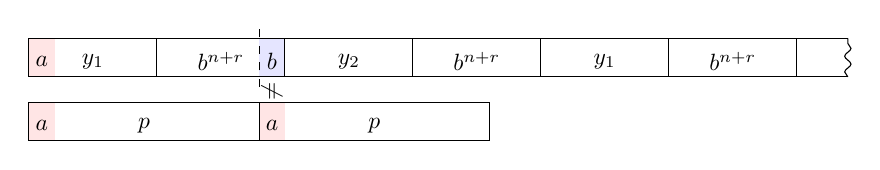
\begin{tikzpicture}[scale=0.65,every node/.style={scale=0.85}]
	\path[fill=red!10] (0,0) rectangle (0.5,0.75);
	\path[fill=red!10] (0,-0.5) rectangle (0.5,-1.25);
	\path[fill=red!10] (4.5,-0.5) rectangle (5,-1.25);
	\path[fill=blue!10] (4.5,0) rectangle (5,0.75);
	
	\draw (0,0) rectangle (15,0.75);
	\draw (0,0) rectangle (15,0.75);
	\draw (15,0) -- (16,0);
	\draw[decorate,decoration={snake,amplitude=.4mm,segment length=2mm}] (16,0) -- (16,0.75);
	\draw (16,0.75) -- (15,0.75);
	
	\draw (2.5,0) -- (2.5,0.75);
	\draw (5,0) -- (5,0.75);
	\draw (7.5,0) -- (7.5,0.75);
	\draw (10,0) -- (10,0.75);
	\draw (12.5,0) -- (12.5,0.75);
	
	\node at (1.25,0.3) {$y_1$};
	\node at (3.75,0.3) {$b^{n+r}$};
	\node at (6.25,0.3) {$y_2$};
	\node at (8.75,0.3) {$b^{n+r}$};
	\node at (11.25,0.3) {$y_1$};
	\node at (13.75,0.3) {$b^{n+r}$};
	
	\draw[dashed] (4.5,-0.2) -- (4.5,0.95);
	
	\node at (4.75,0.3) {$b$};
	\node at (0.25,0.3) {$a$};
	\node at (0.25,-0.95) {$a$};
	\node at (4.75,-0.95) {$a$};
	
	\node[rotate=90] at (4.75,-0.275) {$\neq$};
	
	\draw (0,-0.5) rectangle (4.5,-1.25);
	\draw (4.5,-0.5) rectangle (9,-1.25);
	
	\node at (2.25,-0.95) {$p$};
	\node at (6.75,-0.95) {$p$};
\end{tikzpicture}
				\subcaption{Case $\left\lfloor\frac{|p|}{n+r}\right\rfloor$ is odd\label{fig:repetition:i1}}
			\end{subfigure}
			\begin{subfigure}{\textwidth}
				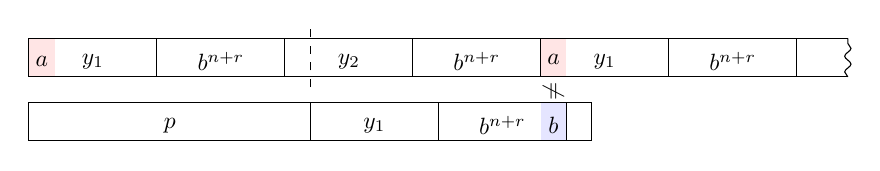
\begin{tikzpicture}[scale=0.65,every node/.style={scale=0.85}]
	\path[fill=red!10] (0,0) rectangle (0.5,0.75);
	\path[fill=blue!10] (10,-0.5) rectangle (10.5,-1.25);
	\path[fill=red!10] (10,0) rectangle (10.5,0.75);
	
	\draw (0,0) rectangle (15,0.75);
	\draw (15,0) -- (16,0);
	\draw[decorate,decoration={snake,amplitude=.4mm,segment length=2mm}] (16,0) -- (16,0.75);
	\draw (16,0.75) -- (15,0.75);
	
	\draw (2.5,0) -- (2.5,0.75);
	\draw (5,0) -- (5,0.75);
	\draw (7.5,0) -- (7.5,0.75);
	\draw (10,0) -- (10,0.75);
	\draw (12.5,0) -- (12.5,0.75);
	
	\node at (1.25,0.3) {$y_1$};
	\node at (3.75,0.3) {$b^{n+r}$};
	\node at (6.25,0.3) {$y_2$};
	\node at (8.75,0.3) {$b^{n+r}$};
	\node at (11.25,0.3) {$y_1$};
	\node at (13.75,0.3) {$b^{n+r}$};
	
	\draw[dashed] (5.5,-0.2) -- (5.5,0.95);
	
	\draw (0,-0.5) rectangle (5.5,-1.25);
	\draw (5.5,-0.5) rectangle (11,-1.25);
	\draw (8,-0.5) -- (8,-1.25);
	\draw (10.5,-0.5) -- (10.5,-1.25);
	
	\node at (2.75,-0.95) {$p$};
	\node at (6.75,-0.95) {$y_1$};
	\node at (9.25,-0.95) {$b^{n+r}$};
	
	\node at (0.25,0.3) {$a$};
	\node at (10.25,0.35) {$a$};
	\node at (10.25,-0.95) {$b$};
	
	\node[rotate=90] at (10.25,-0.275) {$\neq$};
\end{tikzpicture}
				\subcaption{Case $\left\lfloor\frac{|p|}{n+r}\right\rfloor$ is even\label{fig:repetition:i2}}
			\end{subfigure}
			\caption{\label{fig:repetition}}
		\end{figure}
		
		Now, assume $|p|$ is a divisor of $n+r$. Then we can understand the blocks of length $n+r$ as letters of the alphabet $\{b^{n+r},y_1,\dots,y_i\}$. Since there is no $y_i$-block in $v_i$ we have $|p|\geq|v_iy_i|$. Since $p$ starts with $y_1$ and $y_i$ is followed by $b^{n+r}$, $p$ has length at least $|v_ix_i|$.
		
		\emph{Proof of (\ref{prf:short_from_skeleton:i2}).}\ By construction, it is easy to see that $\vec{v}=(v_0,\dots,v_n)$ is a border-decomposition of $v=v_n$. We prove now by induction on $0\leq i<n$ that $(v_0,\dots,v_{i+1})$ is a complete border-decomposition of $v_i$. The case $i=0$ is easy to verify since $v_1\in aA^{r-1}b^{2n+r}$. So, let $i\geq1$. Assume there is $u\in A^*$ with $v_i\presuf u\presuf v_{i+1}$. Let $u$ be of minimal length satisfying this inequality. Then there are two possible cases:
		
		First, suppose $|u|\geq|v_ix_i|$ holds, i.e., the prefix and suffix $u$ overlap in $v_i$ and the overlap contains at most $x_i$ (cf.\ Fig.~\ref{fig:skeleton}). Let $x,y\in A^*$ such that $u=xx_iv_i=y$. Then we have $|x|=|y|$ and $m:=xx_iy\presuf u$. Hence, by minimality of $u$ we have $|m|\leq|v_i|$ and therefore, by induction hypothesis, $m=v_k$ for some $0< k\leq i$. This implies
		\[v_{k-1}x_{k-1}v_{k-1}=v_k=m=xx_iy\,.\]
		Since $|x|=|y|$ and $|x_i|=|x_{k-1}|$ we have $x_i=x_{k-1}$, which is a contradiction to the construction of the $x_i$'s.
		
		\begin{figure}[h]
			\centering\begin{tikzpicture}[scale=0.65,every node/.style={scale=0.85}]
	\node at (-0.75,0.2){$v_{i+1}=$};
	\node at (-0.75,-0.9){$u=$};
	\node at (-0.75,-1.7){$u=$};
	
	\draw (0,0) rectangle (15,0.75);
	\draw (0, -0.5) rectangle (10,-1.25);
	\draw (5, -1.25) rectangle (15,-2);

	\draw (5,.75) -- (5,0);	
	\draw (6,.75) -- (6,0);
	\draw (9,.75) -- (9,0);
	\draw (10,.75) -- (10,0);
	
	\draw (5,-0.5) -- (5,-2);
	\draw (6,-0.5) -- (6,-2);
	\draw (9,-0.5) -- (9,-2);
	\draw (10,-0.5) -- (10,-2);
	
	\node at (7.5,0.3) {$x_i$};
	\node at (9.5,-0.95) {$y$};
	\node at (5.5,-1.7) {$x$};
	
	\draw[snake=brace] (0,0.8) -- (6,0.8);
	\draw[snake=brace] (9,0.8) -- (15,0.8);
	\draw[snake=brace] (10,-2.05) -- (5,-2.05);
	
	\node at (3,1.1) {$v_i$};
	\node at (12,1.1) {$v_i$};
	\node at (7.5,-2.4) {$m$};
\end{tikzpicture}
			\caption{\label{fig:skeleton}}
		\end{figure}
		
		Now, suppose $|u|<|v_ix_i|$. If $|u|\geq\frac{|v_{i+1}|}{2}$ (i.e., the prefix and suffix $u$ in $v_i$ overlap) then there is a word $m\in A^*$ such that $m\presuf u$ holds. Hence, by minimality of $u$ and by induction hypothesis we have $m=v_k$ for some $0\leq k\leq i$. Since $|m|<|x_i|=|x_1|$ we have $m=\varepsilon$, i.e., we have $|u|=\frac{|v_{i+1}|}{2}$.
		
		Suppose $|u|\leq\frac{|v_{i+1}|}{2}$ (i.e., the prefix and suffix $u$ in $v_i$ do not overlap). Then there is a word $p\in A^*$ such that $v_{i+1}=pu$. Since $u$ is a prefix of $v_{i+1}$ and $|p|>\frac{|v_{i+1}|}{2}$, $u$ also is a prefix of $p$. Hence, $p$ is a period of $v_{i+1}$ and we have
		\[|p|=|v_{i+1}|-|u|<|v_{i+1}|-|v_i|=|v_ix_i|\,.\]
		This is a contradiction to property~\ref{prf:short_from_skeleton:i1} stating that $v_ix_i$ is the minimal period of $v_{i+1}$.
		
		So, in both cases we have seen that there is no $v_i\presuf u\presuf v_{i+1}$, i.e., $(v_0,\dots,v_{i+1})$ is a complete border-decomposition.
		
			Finally, let $0\leq i<n$. Then we have
		\[\calS_r(v)[i]=\pref_r(\inv{v_i}v)=\pref_r(\calS_r(w)[i]\,s)=\calS_r(w)[i]\]
		for some $s\in A^*$, i.e., $\calS_r(v)=\calS_r(w)$. Additionally, we have $|v_i|=2|v_{i-1}+2n+2r$ for $1\leq i\leq n$ and $|v_0|=0$ which results in $|v|=|v_n|=(2^n-1)(2n+2r)=\calO(2^{nr})$.
	\end{proof}
	
	\msoth*
	\begin{proof}
		Due to \cite{RobS84} each planar graph is a minor of some grid $\frakG_n$. Since each $\frakG_n$ is an induced subgraph of $\ud{\cQ}$ by Proposition~\ref{prop:grid}, each planar graph is minor of an induced subgraph of $\ud{\cQ}$. Hence, by \cite[Theorem~5]{See91} $\MSOTh{\ud{\cQ}}$ is undecidable. Since $\ud{G}$ is interpretable in $\FOTh{\cQ}$, $\MSOTh{\cQ}$ is undecidable as well.
	\end{proof}

	\decidable*
	\begin{proof}
		We use the standard model-checking algorithm for first-order logic but restrict quantification to the $\exp_{r+1}(2,f(r))$-neighborhood of the current variable assignment. The correctness of this procedure is guaranteed by Corollary \ref{cor:equivalence}.
		We see that the values $|\rd{p}|$ and $|\wrt{p}|$ are bounded by $r\exp_{r+1}(2,f(r))$
		Hence, by Lemma \ref{lem:neighborhood_size} the algorithm needs to consider at most $|A|^{4r} r(\exp_{r+1}(2,f(r)) +1)$ many Elements, which leads to a runtime of
		$|\phi| \cdot (|A|^{4r} r(\exp_{r+1}(2,f(r)) +1))^r$, which is obviously a primitive recursive function. 
	\end{proof}
\end{appendix}
